% no answer key
% \documentclass[letterpaper]{exam}

% answer key
\documentclass[letterpaper, landscape]{exam}
\usepackage{2in1, lscape} 
\printanswers{}

% for the cent symbol
\usepackage{textcomp}

% the textcent command eats the space following the symbol
\usepackage{xspace}
\newcommand{\cent}{\textcent\xspace}

\usepackage{units} 
\usepackage{xfrac} 
\usepackage[fleqn]{amsmath}
\usepackage{cancel}
\usepackage{float}
\usepackage{mdwlist}
\usepackage{booktabs}
\usepackage{cancel}
\usepackage{polynom}
\usepackage{caption}
\usepackage{fullpage}
\usepackage{comment}
\usepackage{enumerate}
\usepackage{graphicx}
\usepackage{parskip}

\everymath{\displaystyle}

\title{Statistics \\ Chapter 17 Homework}
\date{\today}
\author{}

\begin{document}

  \maketitle

  \section{Homework}
  Chapter 17: 25--28, 30--31, 33, 35, 38, 44--45, 47

  \ifprintanswers{}
    \section{Solutions}
    \begin{description}

      \item[25] 
        \begin{align*}
          t_1 &= 0.7490 \\
          t_2 &= 3.2769 \\
        \end{align*}

        From Table C, the first P-value is between 0.4 and 0.5 and the second
        P-value is between 0.01 and 0.005.

      \item[26]
        From Table C, $t^* = 1.984$. This produces a 95\% confidence interval of
        $(26,22, 27.38)$.

      \item[27]
        \begin{enumerate}[(a)]
          \item The sample size of 1470 is big enough that it doesn't matter
            much whether the data has a normal distribution.

          \item From Table C, $t^* = 2.581$. This produces a 99\% confidence
            interval of $(237.16, 242.84)$.

          \item 
            \[
              t = -2.7273
            \]

            From Table C, the one-sided P-value is somewhere between 0.005 and
            0.0025. This is good evidence that the students are below average.

        \end{enumerate}

      \item[28]
        \begin{enumerate}[(a)]
          \item From Table C, $t^* = 2.056$.  The 95\% confidence interval is
            $(111.22, 118.58)$.

          \item
            \begin{itemize*}
              \item The original 54 subjects are randomly selected from the
                white male population.

              \item The study is only advertised as representing white males.

              \item The subjects were randomly selected for the treatment and
                control groups.

              \item Blood pressure has an approximately Normal distribution.
            \end{itemize*}

        \end{enumerate}

      \item[30]
        \begin{figure}[H]
          \centering
          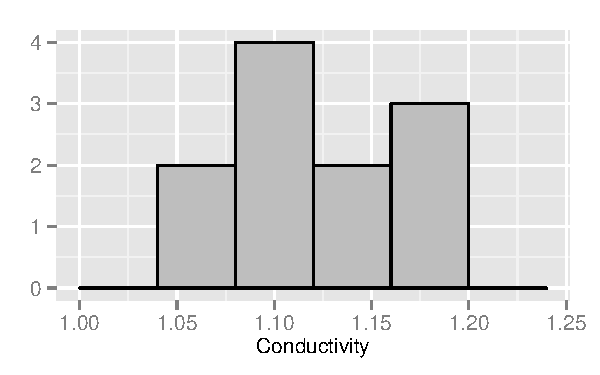
\includegraphics[scale = 1.0]{figures/ex30.pdf}
          \caption{Exercise 30}\label{fig:ex30}
        \end{figure}
        
        \begin{enumerate}[(a)]
          \item See Figure~\ref{fig:ex30}. There aren't very many samples, but
            they look evenly distributed.

          \item
            \begin{align*}
              \bar{x} & = 1.12 \\
              s       & = 0.044 \\
            \end{align*}

            From Table C, $t^* = 2.228$. The confidence interval is:
            \begin{align*}
              \mu & = 1.12 \pm 2.228 \cdot \frac{0.044}{\sqrt{10}} \\
                  & = (1.10, 1.13)
            \end{align*}

          \item
            \[
              t = 8.9538
            \]

            Since all the values are greater than 1, the alternative hypothesis
            should be one sided. From Table C, $P-value < 0.0005$, so it is very
            likely the mean conductivity of this glass is 1.
        \end{enumerate}

      \item[31]
        \begin{figure}[H]
          \centering
          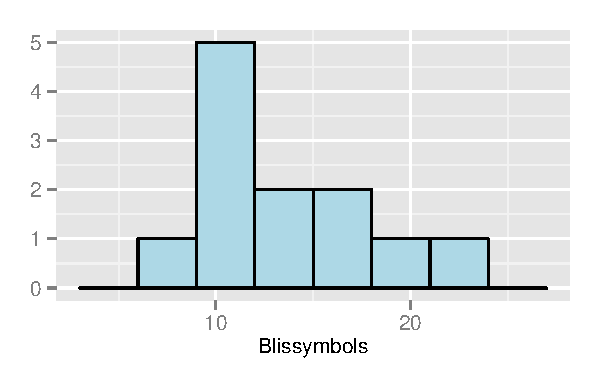
\includegraphics[scale = 1.0]{figures/ex31.pdf}
          \caption{Exercise 31}\label{fig:ex31}
        \end{figure}
        
        \begin{enumerate}[(a)]
          \item See Figure~\ref{fig:ex31}. There aren't very many samples, but
            they look fairly Normal.

          \item
            \begin{align*}
              \bar{x} & = 12.83 \\
              s       & = 4.65 \\
            \end{align*}

            From Table C, $t^* = 1.796$. The confidence interval is:
            \begin{align*}
              \mu & = 12.83 \pm 1.796 \cdot \frac{4.65}{\sqrt{10}} \\
                  & = (10.42, 15.24)
            \end{align*}
        \end{enumerate}

      \item[33]
        \begin{figure}[H]
          \centering
          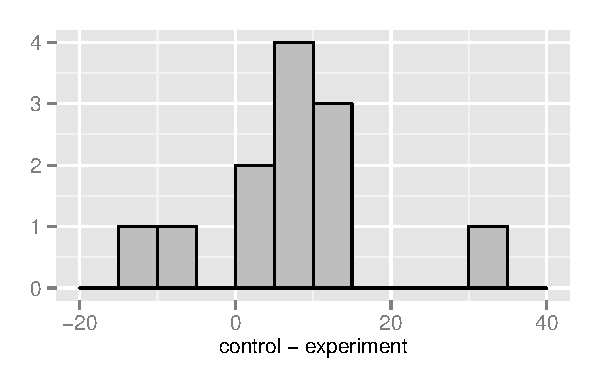
\includegraphics[scale = 1.0]{figures/ex33.pdf}
          \caption{Exercise 33}\label{fig:ex33}
        \end{figure}

        \begin{enumerate}[(a)]
          \item See Figure~\ref{fig:ex33}.

          \item 
            With the outlier, there is a significant difference. Without the
            outlier, there (barely) isn't a significant difference.

            \begin{tabular}[H]{lrr}
              \toprule
                              & t-value & P-value \\
              \midrule
              with outlier    & 2.0761  & 0.031 \\
              without outlier & 1.7881  & 0.052 \\
              \bottomrule
            \end{tabular}

        \end{enumerate}

      \item[35]
        \begin{figure}[H]
          \centering
          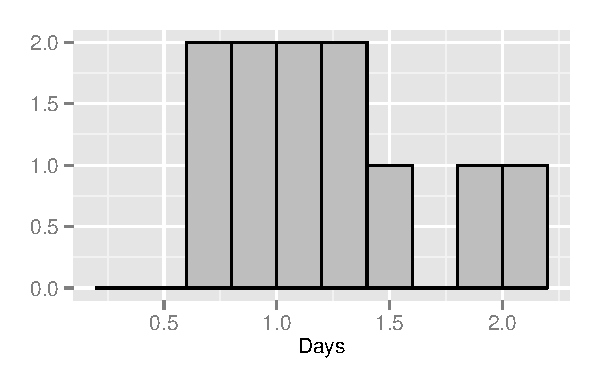
\includegraphics[scale = 1.0]{figures/ex35.pdf}
          \caption{Exercise 35}\label{fig:ex35}
        \end{figure}

        \begin{enumerate}[(a)]
          \item See Figure~\ref{fig:ex35}. 
          \item The 90\% confidence interval is $(0.9210, 1.4244)$.
        \end{enumerate}

      \item[38]
        \begin{enumerate}[(a)]
          \item The spore count varies quite a bit by day. We want to make sure
            we compare the two rooms on the same day, so that the experiment
            isn't measuring differences between days instead of the difference
            between the two rooms.

          \item 
            \begin{align*}
              \bar{x}_{kr}   & = 2138.5 \\
              \bar{x}_{pr}   & = 314 \\
              \bar{x}_{diff} & = 1824.5 \\
              \\
              \mu_{diff} &= (843, 2806) \\
            \end{align*}

          \item The sample size is very small. We can be confident that there
            are more spores in the kill room, but not very precise about how
            many more spores there are on average.

        \end{enumerate}

      \item[44]
        \begin{figure}[H]
          \centering
          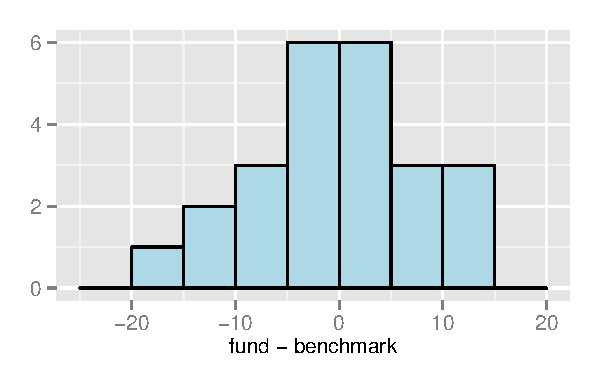
\includegraphics[scale = 1.0]{figures/ex44.pdf}
          \caption{Exercise 44}\label{fig:ex44}
        \end{figure}

        The data looks fairly Normal. See Figure~\ref{fig:ex44}.

        The 95\% confidence interval for the mean difference is $(-3.45, 3.30)$.
        Since this interval contains 0, it doesn't rule out the fund exactly
        matching its benchmark.

        The null hypothesis is that the mean difference is 0 and the alternative
        hypothesis is that the mean difference is non-zero.

        t = -0.0462 which gives a P-value of 0.9636. This doesn't rule out the
        null hypothesis, so there's no reason to think the fund's performance is
        different from its benchmark.
        
      \item[45]
        \begin{figure}[H]
          \centering
          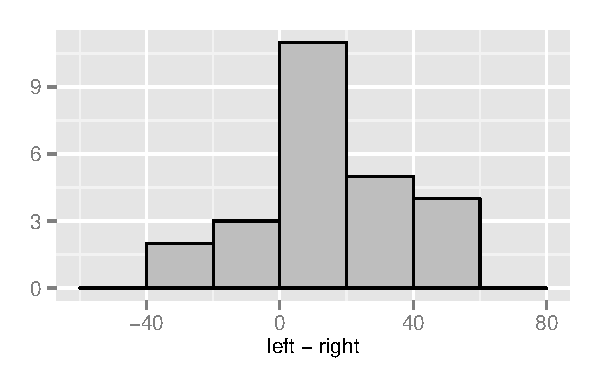
\includegraphics[scale = 1.0]{figures/ex45.pdf}
          \caption{Exercise 45}\label{fig:ex45}
        \end{figure}

        The data looks fairly Normal. See Figure~\ref{fig:ex45}.

        The null hypothesis is that the mean difference is 0 and the alternative
        hypothesis is that the mean difference is greater than zero. We should
        use a one-sided t-test.

        t = 2.9037 which gives a one-sided P-value of 0.0.0078. There is a
        statistically significant difference at the $\alpha = 0.05$ level.
        
      \item[47]

        \paragraph{Approach 1}

        \begin{align*}
          \bar{x}_{right} &= \unit[104.12]{s} \\
          \bar{x}_{left} &= \unit[117.44]{s} \\
        \end{align*}

        The right hand threads only take 89\% of the time of the left hand
        threads.

        \paragraph{Approach 2}
        It looks like the task takes around 2 minutes, so a worker could do
        about 30 tasks per hour working steadily. 

        If a worker worked 40 hours per week and spent half his time on this
        kind of task, he would do approximately $20 \cdot 30 \approx 600$ tasks
        per week. 
        
        If a worker typically worked 50 weeks per year, he would do about $600
        \cdot 50 = 30,000$ tasks per year.

        The 90\% confidence interval for the mean difference is $(5.47, 21.17)$.

        If we save 5 to 21 seconds per task, we could save 40 to 175 hours per
        worker per year. 

        This means we could give everybody an extra 1 to 4 weeks of vacation a
        year and still make the same amount of stuff.

  \end{description}

  \else
    \vspace{12 cm}
    \begin{quote}
      \begin{em}
        Everything goes, everything returns; eternally rolls the wheel of
        being.
      \end{em}
    \end{quote}
    \hspace{1 cm}--Frederich Nietzsche
  \fi

\end{document}

